% !TEX TS-program = xelatex
% !TEX encoding = UTF-8 Unicode
\documentclass[12pt,a4paper]{article}

\IfFileExists{src/libs/body.tex}{% --- body.tex ---
\usepackage{pdfpages}
\usepackage{fontspec}
% Prefer Times New Roman when available; fall back in container environments.
\IfFontExistsTF{Times New Roman}{
  \setmainfont{Times New Roman}
}{
  \setmainfont{Liberation Serif}
}
\usepackage[vietnamese]{babel}

% Page layout and spacing
\usepackage[left=3cm,right=2cm,top=2cm,bottom=2cm]{geometry}
\usepackage{titlesec}
\usepackage{setspace}

% Silence noisy warnings
\usepackage{silence}
\WarningFilter{transparent}{Loading aborted}
\WarningFilter{hyperref}{The anchor of a bookmark and its parent's}

% Core packages
\usepackage{float}
\usepackage{svg}
\usepackage{graphicx}
\graphicspath{{assets/}{../assets/}{../../assets/}}
\svgpath{{assets/}{../assets/}{../../assets/}}
\usepackage{enumitem}
\usepackage{array}
\usepackage{tabularx}
\usepackage{multirow}
\usepackage[table]{xcolor}
\usepackage{ulem}
\usepackage{xurl}

% ====== THÊM 2 GÓI NÀY ĐỂ FIX LỖI ADJUSTBOX VÀ FOREST ======
\usepackage{adjustbox}
\usepackage[edges]{forest}
% ============================================================

% TikZ
\usepackage{tikz}

% ====== BỔ SUNG FIT, BACKGROUNDS, TREES VÀO DANH SÁCH ======
\usetikzlibrary{calc, arrows.meta, shapes.geometric, positioning, fit, backgrounds, trees}

% Table tuning
\renewcommand{\tabularxcolumn}[1]{m{#1}}
\hbadness=10000
\hfuzz=10000pt

% Shared commands
\newcommand{\subsecheading}[1]{%
    \par\vspace{2pt}%
    \hspace{1.5em}\textbf{#1}%
    \par\vspace{2pt}%
}
\newcommand{\introtext}[1]{%
    \par\hspace{3.0em}#1\par%
}
\newcommand{\StandaloneDocumentSetup}[2]{%
  \pagenumbering{arabic}%
  \ApplyStandardFooter{#1}{#2}%
}
\newcommand{\StandaloneSectionSetup}[2]{%
  \ApplyStandardFooter{#1}{#2}%
}

% Math
\usepackage{amsmath}

% Hyperref
\usepackage{hyperref}
\hypersetup{
    colorlinks=true,
    linkcolor=black,
    filecolor=magenta,
    urlcolor=blue,
}}{% --- body.tex ---
\usepackage{pdfpages}
\usepackage{fontspec}
% Prefer Times New Roman when available; fall back in container environments.
\IfFontExistsTF{Times New Roman}{
  \setmainfont{Times New Roman}
}{
  \setmainfont{Liberation Serif}
}
\usepackage[vietnamese]{babel}

% Page layout and spacing
\usepackage[left=3cm,right=2cm,top=2cm,bottom=2cm]{geometry}
\usepackage{titlesec}
\usepackage{setspace}

% Silence noisy warnings
\usepackage{silence}
\WarningFilter{transparent}{Loading aborted}
\WarningFilter{hyperref}{The anchor of a bookmark and its parent's}

% Core packages
\usepackage{float}
\usepackage{svg}
\usepackage{graphicx}
\graphicspath{{assets/}{../assets/}{../../assets/}}
\svgpath{{assets/}{../assets/}{../../assets/}}
\usepackage{enumitem}
\usepackage{array}
\usepackage{tabularx}
\usepackage{multirow}
\usepackage[table]{xcolor}
\usepackage{ulem}
\usepackage{xurl}

% ====== THÊM 2 GÓI NÀY ĐỂ FIX LỖI ADJUSTBOX VÀ FOREST ======
\usepackage{adjustbox}
\usepackage[edges]{forest}
% ============================================================

% TikZ
\usepackage{tikz}

% ====== BỔ SUNG FIT, BACKGROUNDS, TREES VÀO DANH SÁCH ======
\usetikzlibrary{calc, arrows.meta, shapes.geometric, positioning, fit, backgrounds, trees}

% Table tuning
\renewcommand{\tabularxcolumn}[1]{m{#1}}
\hbadness=10000
\hfuzz=10000pt

% Shared commands
\newcommand{\subsecheading}[1]{%
    \par\vspace{2pt}%
    \hspace{1.5em}\textbf{#1}%
    \par\vspace{2pt}%
}
\newcommand{\introtext}[1]{%
    \par\hspace{3.0em}#1\par%
}
\newcommand{\StandaloneDocumentSetup}[2]{%
  \pagenumbering{arabic}%
  \ApplyStandardFooter{#1}{#2}%
}
\newcommand{\StandaloneSectionSetup}[2]{%
  \ApplyStandardFooter{#1}{#2}%
}

% Math
\usepackage{amsmath}

% Hyperref
\usepackage{hyperref}
\hypersetup{
    colorlinks=true,
    linkcolor=black,
    filecolor=magenta,
    urlcolor=blue,
}}
\IfFileExists{src/libs/header.tex}{% --- header.tex ---
\usepackage{fancyhdr}
\setlength{\headheight}{15.5pt} % Thêm dòng này để fix cảnh báo chiều cao
%\setlength{\headheight}{14.5pt}
\addtolength{\topmargin}{-2.5pt}

\pagestyle{fancy}
\fancyhf{}
\renewcommand{\headrulewidth}{0pt}
\renewcommand{\footrulewidth}{0pt}

\newcommand{\ApplyStandardHeader}{%
  \fancyhead[L]{%
    \begin{minipage}[t]{0.795\linewidth}%
      UIT \textbar{} SS004.F21 \textbar{} Nhóm 03 \textbar{} Đồ án cuối kỳ%
    \end{minipage}%
    \vrule%
    \begin{minipage}[t]{0.185\linewidth}%
      \centering cTetris%
    \end{minipage}%
  }%
}

\ApplyStandardHeader
}{% --- header.tex ---
\usepackage{fancyhdr}
\setlength{\headheight}{15.5pt} % Thêm dòng này để fix cảnh báo chiều cao
%\setlength{\headheight}{14.5pt}
\addtolength{\topmargin}{-2.5pt}

\pagestyle{fancy}
\fancyhf{}
\renewcommand{\headrulewidth}{0pt}
\renewcommand{\footrulewidth}{0pt}

\newcommand{\ApplyStandardHeader}{%
  \fancyhead[L]{%
    \begin{minipage}[t]{0.795\linewidth}%
      UIT \textbar{} SS004.F21 \textbar{} Nhóm 03 \textbar{} Đồ án cuối kỳ%
    \end{minipage}%
    \vrule%
    \begin{minipage}[t]{0.185\linewidth}%
      \centering cTetris%
    \end{minipage}%
  }%
}

\ApplyStandardHeader
}
\IfFileExists{src/libs/footer.tex}{% --- footer.tex ---
\usepackage{lastpage}

\newcommand{\ApplyStandardFooter}[2]{%
  \fancyfoot[L]{%
    \begin{minipage}[t]{0.795\linewidth}%
      Document ID: #1%
    \end{minipage}%
    \vrule%
    \begin{minipage}[t]{0.185\linewidth}%
      \centering\thepage/\pageref{#2}%
    \end{minipage}%
  }%
  \fancypagestyle{plain}{%
    \fancyhf{}%
    \renewcommand{\headrulewidth}{0pt}%
    \renewcommand{\footrulewidth}{0pt}%
    \ApplyStandardHeader%
    \fancyfoot[L]{%
      \begin{minipage}[t]{0.795\linewidth}%
        Document ID: #1%
      \end{minipage}%
      \vrule%
      \begin{minipage}[t]{0.185\linewidth}%
        \centering\thepage/\pageref{#2}%
      \end{minipage}%
    }%
  }%
  \pagestyle{fancy}%
}
}{% --- footer.tex ---
\usepackage{lastpage}

\newcommand{\ApplyStandardFooter}[2]{%
  \fancyfoot[L]{%
    \begin{minipage}[t]{0.795\linewidth}%
      Document ID: #1%
    \end{minipage}%
    \vrule%
    \begin{minipage}[t]{0.185\linewidth}%
      \centering\thepage/\pageref{#2}%
    \end{minipage}%
  }%
  \fancypagestyle{plain}{%
    \fancyhf{}%
    \renewcommand{\headrulewidth}{0pt}%
    \renewcommand{\footrulewidth}{0pt}%
    \ApplyStandardHeader%
    \fancyfoot[L]{%
      \begin{minipage}[t]{0.795\linewidth}%
        Document ID: #1%
      \end{minipage}%
      \vrule%
      \begin{minipage}[t]{0.185\linewidth}%
        \centering\thepage/\pageref{#2}%
      \end{minipage}%
    }%
  }%
  \pagestyle{fancy}%
}
}
\usepackage{docmute}
\hypersetup{pdftitle={Hướng dẫn sử dụng tính năng cốt truyện}}

\begin{document}
\providecommand{\StandaloneSectionSetup}[2]{\ApplyStandardFooter{#1}{#2}}
\StandaloneSectionSetup{08-gameStoryGuide.tex}{LastPageGameStoryGuide}
\onehalfspacing

\section{Hướng dẫn sử dụng tính năng cốt truyện}

\subsection{Tổng quan}
\textbf{gameStory} là màn hình \emph{mở đầu} của ứng dụng \textit{cTetris} -- một đoạn intro ngắn kéo dài 8 giây, đóng vai trò chào mừng người dùng trước khi chuyển đến màn hình điều khiển chính. Đây là màn hình \textbf{đầu tiên} xuất hiện mỗi khi khởi động ứng dụng, giúp hệ thống hoàn tất các thiết lập cần thiết trong lúc bạn quan sát hiệu ứng.

\noindent\textit{Đặc điểm quan trọng ở phiên bản v1:} gameStory vận hành \textbf{hoàn toàn tự động}. Bạn không cần thực hiện bất kỳ thao tác phím hay nhấp chuột nào; ứng dụng sẽ tự động chuyển cảnh ngay khi đoạn intro kết thúc.

\begin{figure}[htbp]
    \centering
    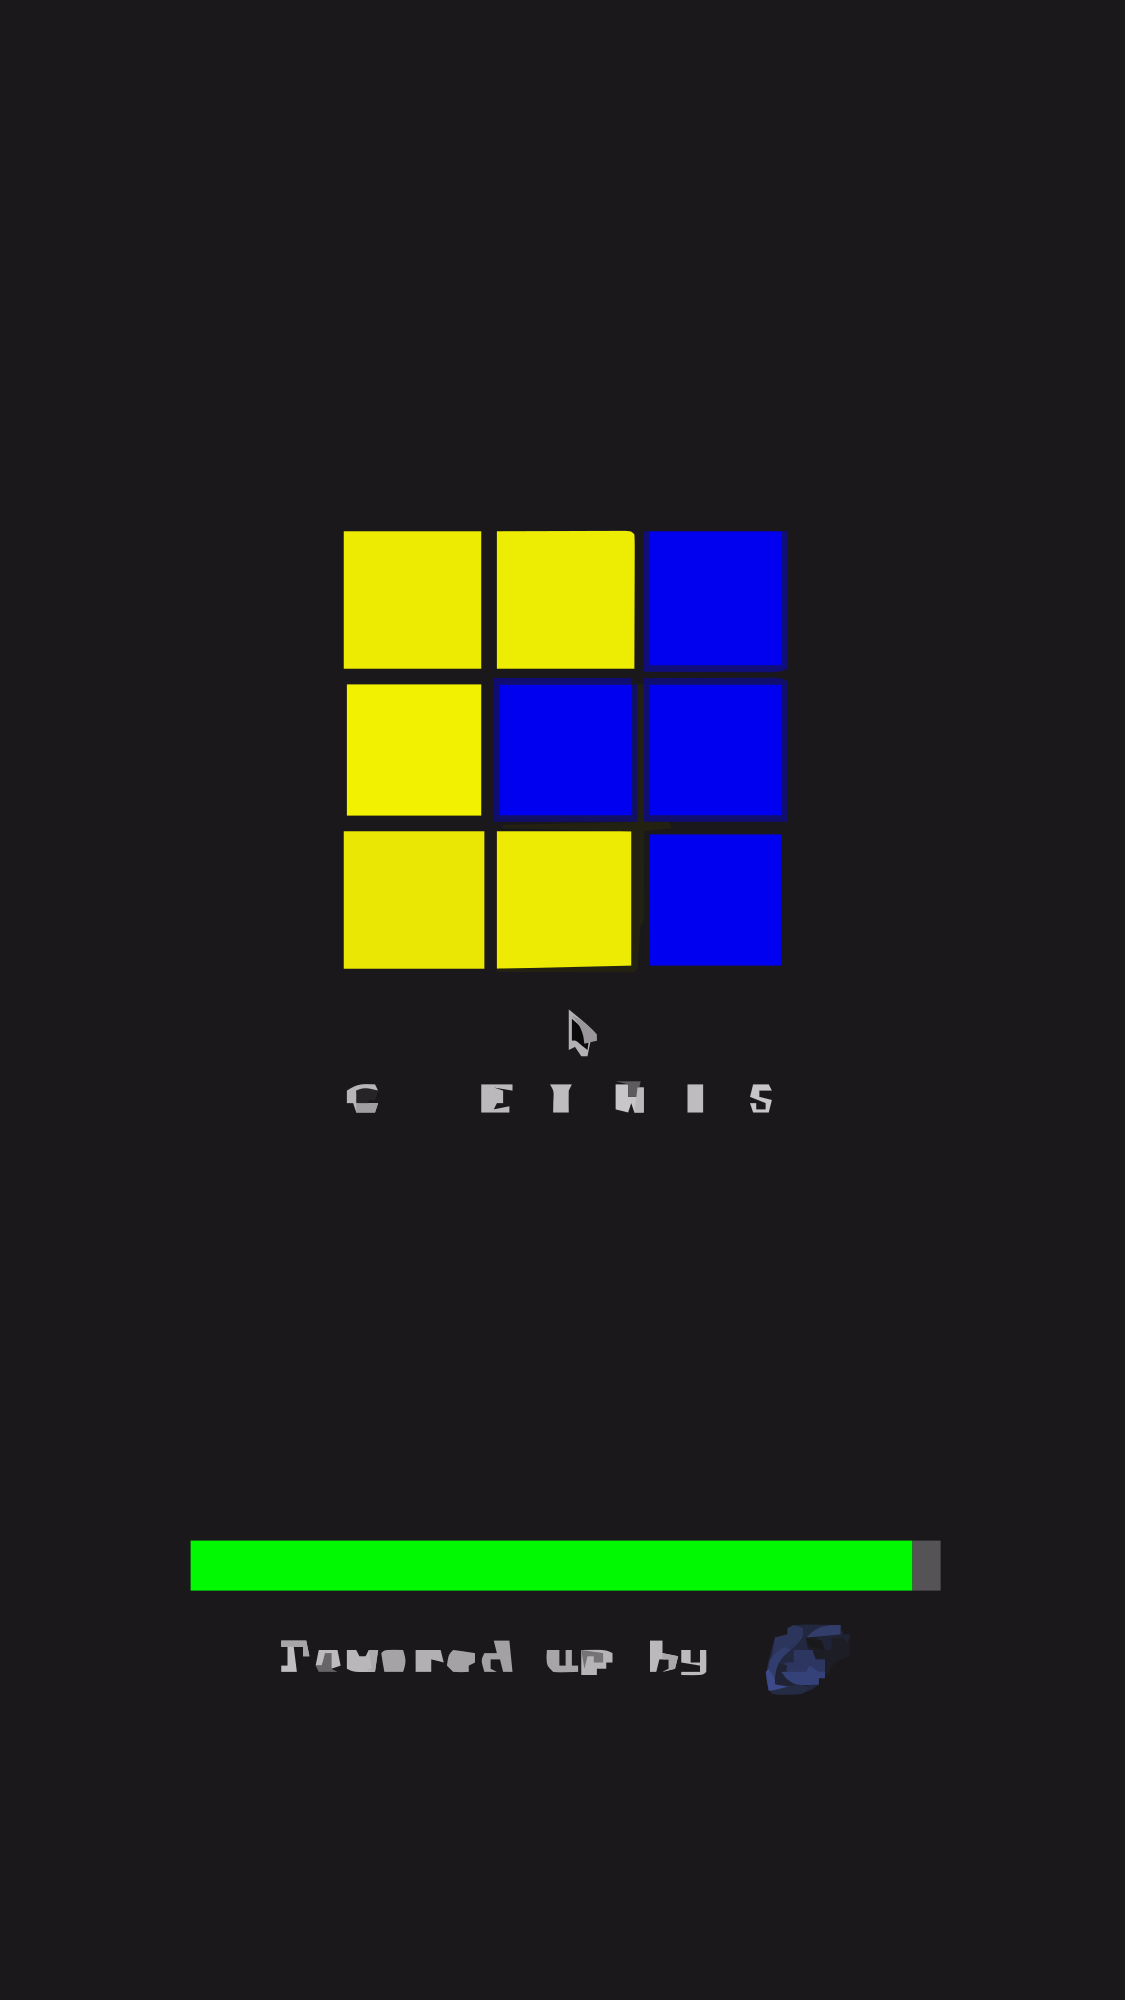
\includegraphics[width=0.3\textwidth]{08-gameStoryGuide-screenshot}
    \\[10pt] % Tạo khoảng cách nhỏ giữa hình và chú thích
    \textit{\small Hình 8.1: Màn hình module gameStory}
\end{figure}

\subsection{Bố cục màn hình}
Toàn bộ màn hình intro nằm gọn trong khung tỉ lệ 9:16 (portrait), nền màu tối, gồm \textbf{ba thành phần thị giác} xếp chồng theo chiều dọc từ trên xuống:

\begin{itemize}
    \item \textbf{Logo cTetris} (vùng giữa màn hình, hơi lệch lên trên) -- biểu tượng 3$\times$3 ô vuông nhiều màu theo phong cách Tetris, kèm dòng chữ \texttt{C T E T R I S} ngay bên dưới.
    \item \textbf{Loading bar} (dưới logo) -- thanh tiến trình màu xanh lá kích thước 180$\times$12 px, lấp đầy dần đều theo thời gian.
    \item \textbf{Dòng credit} (cuối màn hình) -- dòng chữ \texttt{Powered up by} kèm logo nhỏ của Đại học UIT, ghi nhận đơn vị phát triển.
\end{itemize}

\noindent\textit{Mẹo nhận diện:} cả ba thành phần đều xuất hiện đồng bộ với hiệu ứng \emph{fade-in} -- mờ ở giây đầu tiên rồi rõ dần đến cuối, tạo cảm giác chuyển động mượt mà và thống nhất.

\subsection{Hành trình 8 giây của intro}
Khoảng thời gian intro được chia thành các mốc thị giác để bạn dễ hình dung tiến độ:

\vspace{4pt}
\begin{tabularx}{\linewidth}{|l|X|}
    \hline
    \textbf{Thời điểm} & \textbf{Bạn sẽ thấy gì trên màn hình} \\
    \hline
    \texttt{0 giây}    & Màn hình đen, các thành phần bắt đầu xuất hiện rất mờ. \\
    \hline
    \texttt{2 giây}    & Logo cTetris đã rõ khoảng 25\%, loading bar lấp 1/4. \\
    \hline
    \texttt{4 giây}    & Logo và dòng credit hiện rõ 50\%, loading bar đến giữa. \\
    \hline
    \texttt{6 giây}    & Toàn bộ màn hình hiển thị rõ 75\%, loading bar gần đầy. \\
    \hline
    \texttt{8 giây}    & Mọi thành phần đạt độ rõ tối đa, loading bar lấp đầy hoàn toàn. \\
    \hline
    \texttt{> 8 giây}  & Tự động chuyển sang màn hình \textit{gameConsole} (menu chính). \\
    \hline
\end{tabularx}

\vspace{4pt}
\noindent Thời lượng intro được giữ cố định ở \textbf{8 giây} thay vì 3 giây như bản nháp ban đầu, vì hai lý do thực dụng: cho người chơi đủ thời gian nhận biết thương hiệu, và đảm bảo các tài nguyên cần tải qua mạng (trên bản web) kịp sẵn sàng trước khi vào menu.

\subsection{Tương tác trong gameStory}
\textbf{Phiên bản v1 không hỗ trợ thao tác bàn phím, chuột hay cảm ứng} bên trong gameStory -- đây là chủ ý thiết kế, không phải thiếu sót. Mọi phím bấm hoặc click bạn thực hiện trong 8 giây này sẽ \textbf{không có tác dụng}.

Tuy nhiên, bạn vẫn có \emph{một} cách duy nhất để dừng intro lại: \textbf{đóng cửa sổ ứng dụng} bằng nút X của hệ điều hành (hoặc \texttt{Cmd+Q} trên macOS / \texttt{Alt+F4} trên Windows). Khi đó, ứng dụng sẽ thoát ngay lập tức.

\subsection{Khác biệt giữa các nền tảng}
gameStory hoạt động giống nhau về mặt thị giác trên cả hai môi trường, nhưng có vài chi tiết kỹ thuật bạn nên biết:

\vspace{4pt}
\begin{tabularx}{\linewidth}{|l|X|}
    \hline
    \textbf{Yếu tố} & \textbf{Hành vi} \\
    \hline
    Tiêu đề cửa sổ & Trên thanh tiêu đề OS (Desktop) hoặc tab (Web), bạn sẽ thấy \texttt{cTetris ©}. Ký tự \texttt{©} được hệ điều hành / trình duyệt vẽ trực tiếp, không phải canvas của game. \\
    \hline
    Logo và credit  & Đều được tạo bằng đồ họa vector (SVG), nhúng sẵn trong ứng dụng. Vì vậy intro hoạt động ngay cả khi bạn \textbf{không có kết nối Internet}. \\
    \hline
    Tốc độ tải lần đầu & Trên web (WASM), lần khởi động đầu tiên có thể mất thêm vài giây để trình duyệt tải tài nguyên ứng dụng. Loading bar 8 giây giúp bạn không cảm thấy ứng dụng bị treo. \\
    \hline
\end{tabularx}

\subsection{Sau khi intro kết thúc}
Khi loading bar lấp đầy, ứng dụng \textbf{tự động chuyển} sang màn hình \textit{gameConsole} (menu chính). Bạn không cần nhấn phím xác nhận. Tại gameConsole, bạn sẽ thấy bốn nút điều khiển chính: GUIDE, BOARD, PLAY, QUIT.

\noindent\fbox{\begin{minipage}{0.95\linewidth}
\textit{Tham khảo chéo:} mọi hướng dẫn về điều hướng trong menu chính, các popup, scrollbar, và cách bắt đầu ván chơi đã được trình bày đầy đủ trong tài liệu \texttt{09-gameConsoleGuide} (mục \emph{Hướng dẫn sử dụng tính năng cấu hình}). Hướng dẫn về cách chơi trong ván đấu nằm ở \texttt{10-gameCoreGuide} (mục \emph{Hướng dẫn sử dụng tính năng chính}).
\end{minipage}}

\subsection{Mẹo cho lần đầu chơi}
\begin{itemize}
    \item Khi bạn quay lại menu (gameConsole) từ một ván đấu, ứng dụng \textbf{không} chạy lại gameStory -- intro chỉ xuất hiện đúng một lần ở đầu phiên.
    \item Trên web, nếu bạn thấy gameStory chạy lâu hơn 8 giây, đó là do trình duyệt vẫn đang tải tài nguyên. Đợi thêm chút là vào được menu.
    \item Nếu bạn muốn xem lại intro, chỉ cần đóng và mở lại ứng dụng (trên web: \texttt{F5} để tải lại trang).
\end{itemize}

\subsection{Giới hạn của phiên bản v1}
Để bạn nắm rõ kỳ vọng, dưới đây là những điểm \emph{chưa có} trong v1 nhưng đã nằm trong kế hoạch phát triển:
\begin{itemize}
    \item \textbf{Hệ thống hội thoại dẫn truyện} (dialogue) với hiệu ứng chữ chạy kiểu máy đánh chữ -- người chơi sẽ có thể nhấn \texttt{SPACE} / \texttt{ENTER} để bỏ qua hiệu ứng hoặc chuyển dòng.
    \item \textbf{Nút Skip} cho phép người chơi đã quen với intro bỏ qua và vào thẳng menu.
    \item \textbf{Hai nhánh kịch bản} (route A / route B) tạo trải nghiệm khác nhau giữa các lần chơi.
    \item \textbf{Tự động lưu tiến trình} khi hoàn tất một đoạn cốt truyện.
    \item \textbf{Tải tài nguyên qua mạng} cho phép cập nhật hình ảnh, âm thanh và cốt truyện mới mà không cần cài đặt lại ứng dụng.
\end{itemize}
Các tính năng trên sẽ lần lượt xuất hiện ở các phiên bản v2 và v3. Trong v1, gameStory được thiết kế gọn nhẹ và đáng tin cậy -- ưu tiên cho việc khởi động ứng dụng được mượt mà trên cả Desktop lẫn Web.

\label{LastPageGameStoryGuide}
\end{document}